\subsection{Проблема дисбалансу класів}

{
\color{red}
Проблема дисбалансу класів.

The problem of class imbalance in machine learning refers to situations where the number of observations in one class is significantly lower than the number of observations in another class. This can lead to biased models that perform poorly in predicting the underrepresented class. 

For example, in a binary classification problem where the positive class represents only 10% of the data, a model trained on this dataset will have a tendency to predict the negative class for most observations, as this will result in a high overall accuracy.

There are several methods that can be used to address the issue of class imbalance:
\begin{enumerate}
    \item Resampling: This involves either oversampling the minority class or undersampling the majority class to balance the number of observations in each class. This can be done randomly or using more sophisticated methods such as SMOTE (Synthetic Minority Over-sampling Technique).
    \item Cost-sensitive learning: This involves assigning different misclassification costs to each class. In the case of class imbalance, the cost of misclassifying the minority class is typically higher than the cost of misclassifying the majority class. By adjusting the cost matrix, the model can be trained to be more sensitive to the minority class.
    \item Algorithmic adjustments: Some machine learning algorithms have parameters that can be tuned to address class imbalance, such as adjusting the threshold for classification or changing the decision boundary.
    \item Ensemble methods: Ensemble methods such as bagging or boosting can be used to improve the performance of models on imbalanced datasets. By combining multiple models trained on resampled data or with different cost-sensitive learning techniques, the final model can be more robust and accurate.

\end{enumerate}
    

It is important to note that the best method to use for addressing class imbalance depends on the specific dataset and the problem at hand. A thorough understanding of the data and the goals of the analysis is necessary to choose the most appropriate method.

\subsubsection{Upsampling}

\begin{figure}[htbp]
    \centerline{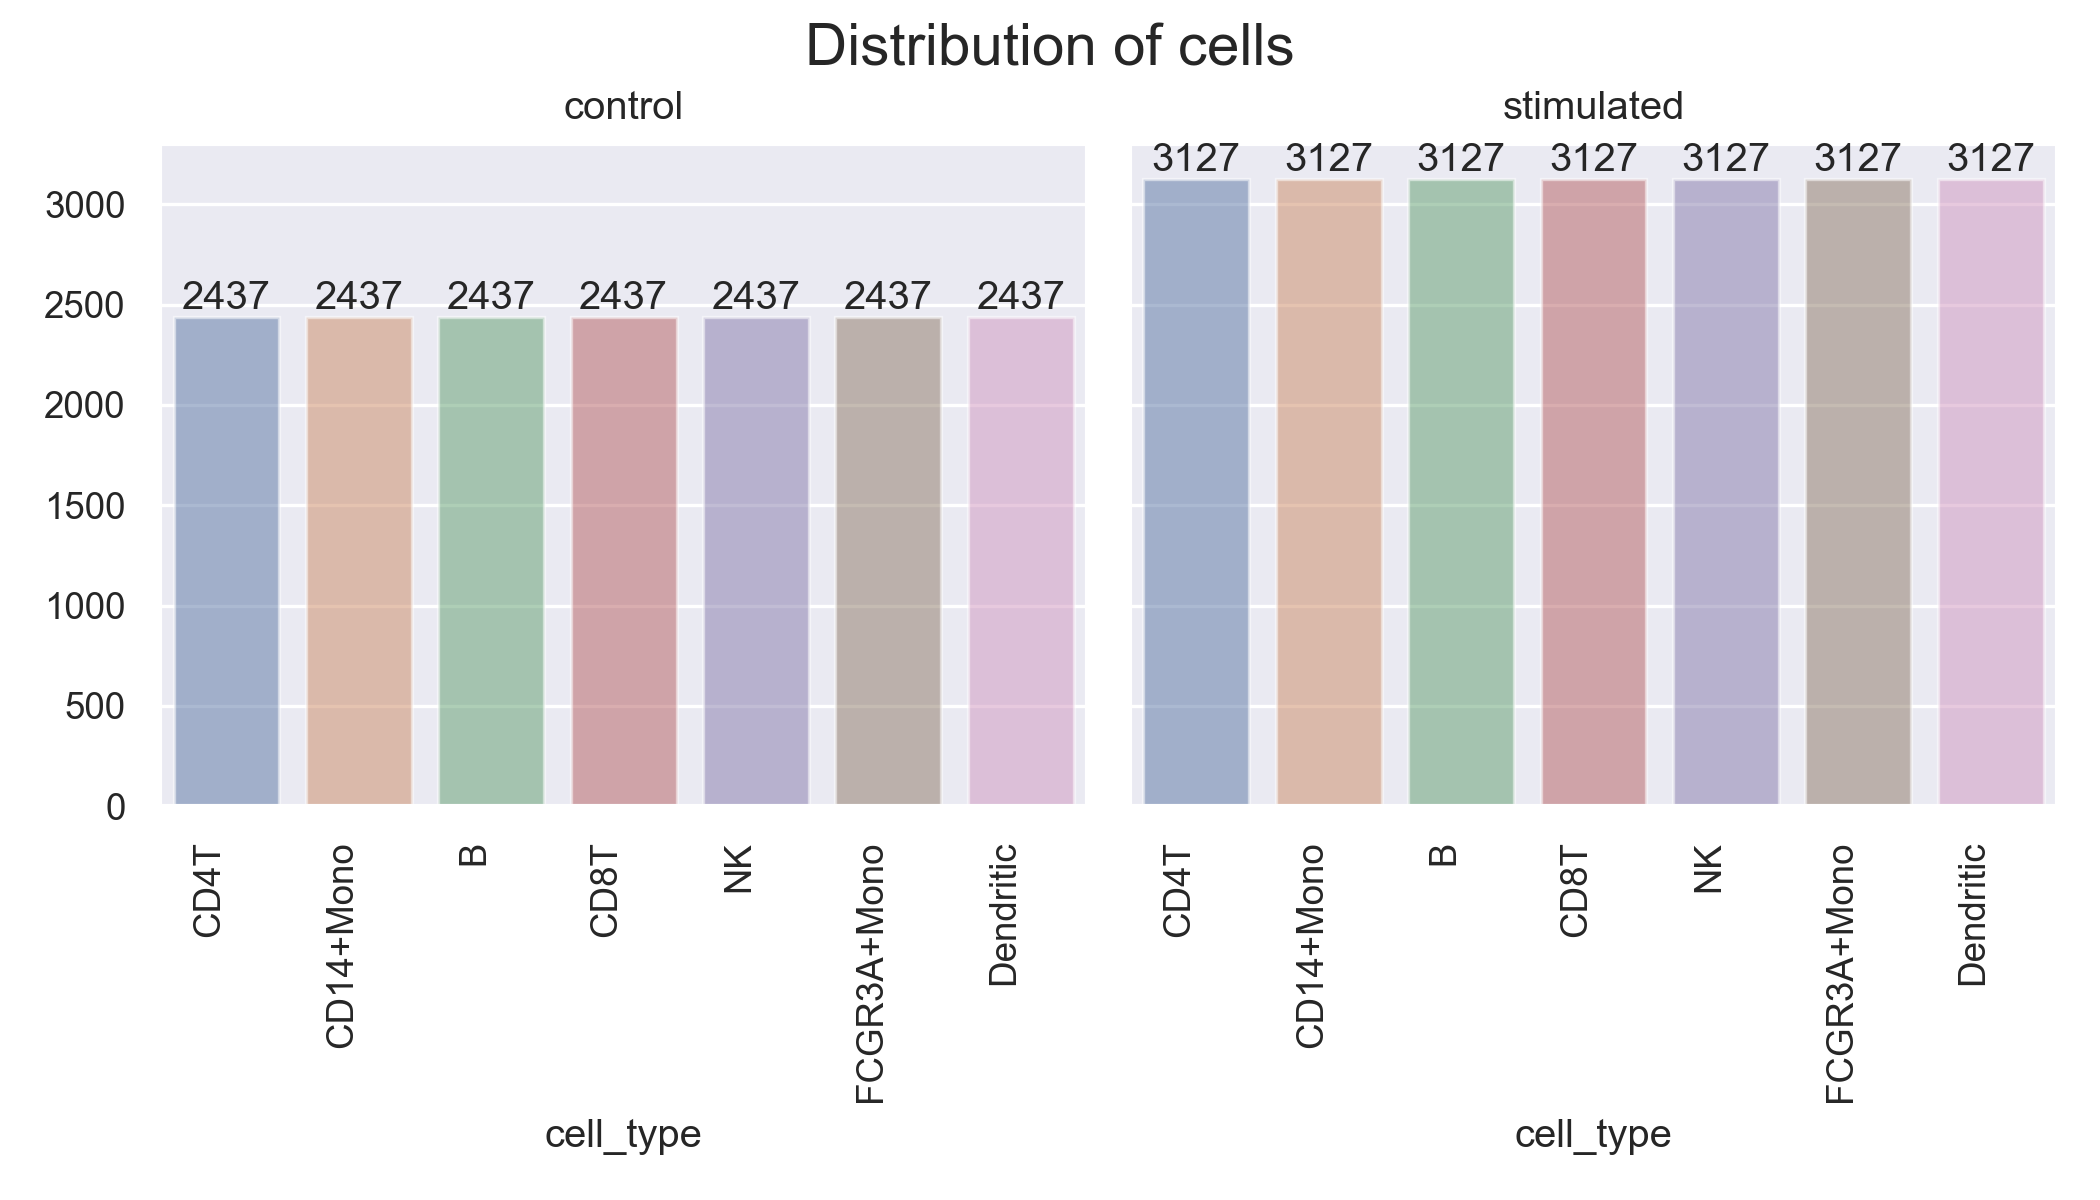
\includegraphics[width=0.6\columnwidth]{pictures/upsampled-dataset.png}}
    \caption{The distribution of cells by classes after upsampling.}
    \label{dataset-cell-types}
\end{figure}

\subsubsection{Downsampling}

\begin{figure}[htbp]
    \centerline{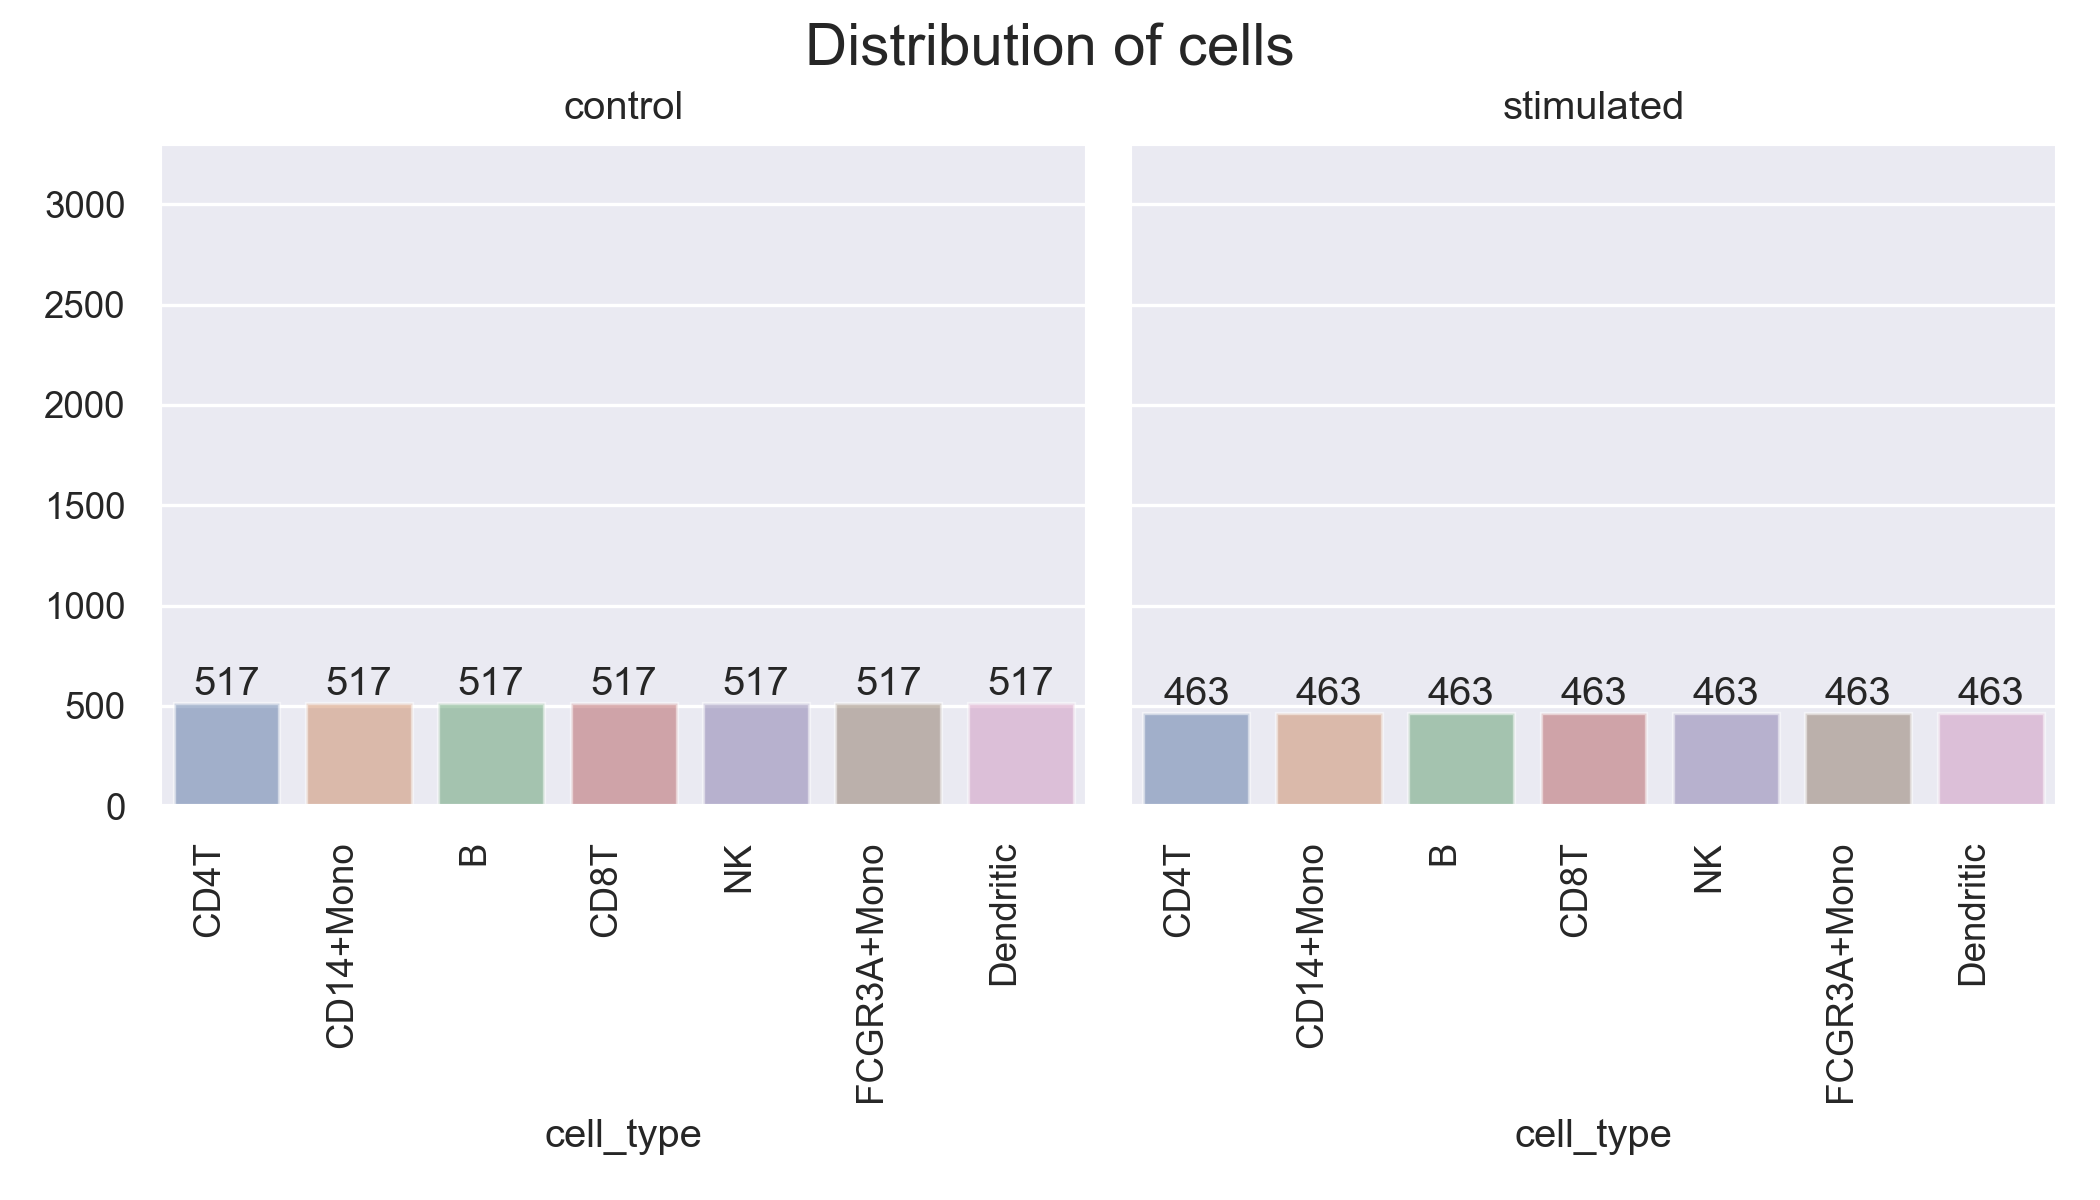
\includegraphics[width=0.6\columnwidth]{pictures/downsampled-dataset.png}}
    \caption{The distribution of cells by classes after downsampling.}
    \label{dataset-cell-types}
\end{figure}
}